\documentclass[tikz,border=5pt]{standalone}
\usepackage{fontspec}
\setmainfont{Times New Roman}
\usepackage{unicode-math}
\setmathfont{Cambria Math}
\usetikzlibrary{shapes.geometric,shapes.misc,positioning,fit,backgrounds,arrows.meta,calc}

\begin{document}
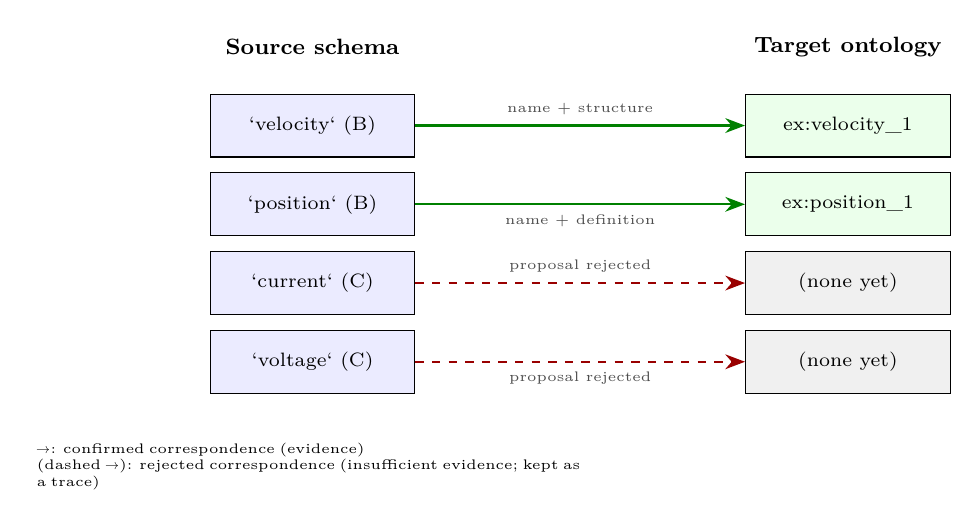
\begin{tikzpicture}[
    node distance=1.2cm and 1.6cm,
    box/.style={rectangle, draw, minimum width=2.6cm, minimum height=0.8cm, align=center, font=\scriptsize},
    label/.style={font=\scriptsize\itshape, text=gray!60!black},
    arrow/.style={-{Stealth[length=2.5mm]}, thick},
    phase/.style={font=\footnotesize\bfseries},
]

% ====== Source schemas ======
\node[phase, font=\footnotesize\bfseries] (sTitle) at (-3.4, 4.2) {Source schema};
\node[box, fill=blue!8] (sB1) at (-3.4, 3.2) {`velocity` (B)};
\node[box, fill=blue!8] (sB2) at (-3.4, 2.2) {`position` (B)};
\node[box, fill=blue!8] (sC1) at (-3.4, 1.2) {`current` (C)};
\node[box, fill=blue!8] (sC2) at (-3.4, 0.2) {`voltage` (C)};

% ====== Canonical target ======
\node[phase, font=\footnotesize\bfseries] (tTitle) at (3.4, 4.2) {Target ontology};
\node[box, fill=green!8] (t1) at (3.4, 3.2) {ex:velocity\_1};
\node[box, fill=green!8] (t2) at (3.4, 2.2) {ex:position\_1};
\node[box, fill=gray!12] (t3) at (3.4, 1.2) {(none yet)};
\node[box, fill=gray!12] (t4) at (3.4, 0.2) {(none yet)};

% ====== Correspondence arrows ======
\draw[arrow, green!50!black] (sB1) -- node[label, above, font=\tiny] {name + structure} (t1);
\draw[arrow, green!50!black] (sB2) -- node[label, below, font=\tiny] {name + definition} (t2);
\draw[arrow, red!60!black, dashed] (sC1) -- node[label, above, font=\tiny] {proposal rejected} (t3);
\draw[arrow, red!60!black, dashed] (sC2) -- node[label, below, font=\tiny] {proposal rejected} (t4);

% ====== Legend ======
\node[font=\tiny, align=left, text width=7cm, below=0.5cm of sC2]
{$\rightarrow$: confirmed correspondence (evidence)\\
(dashed $\rightarrow$): rejected correspondence (insufficient evidence; kept as a trace)};

\end{tikzpicture}
\end{document}
